% pdflatex abra.tex
% convert -density 300x300 -alpha off abra.pdf abra.png
\documentclass[border={2pt 2pt 2pt 2pt}]{standalone}
\usepackage{tikz}
\usetikzlibrary{calc}
\begin{document}

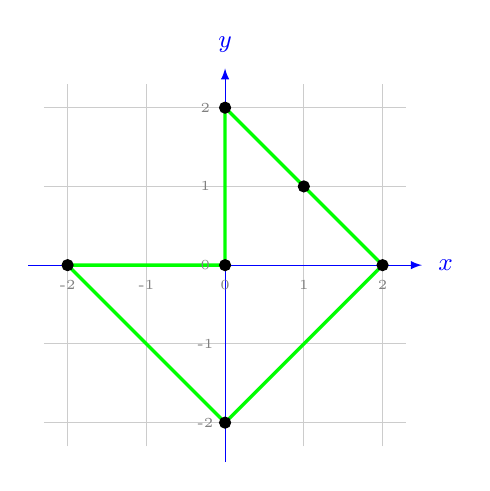
\begin{tikzpicture}
\draw[thin,black!20] (-2.3,-2.3) grid (2.3,2.3);
\draw[thin,blue,-latex] (-2.5,0) -- (2.5,0);
\node[blue] at (2.8,0) {\small$x$};
\draw[thin,blue,-latex] (0,-2.5) -- (0,2.5);
\node[blue] at (0,2.8) {\small$y$};
\draw[very thick,green] (0,0)--(-2,0)--(0,-2)--(2,0)--(1,1)--(0,2)--cycle;
\filldraw[black] (2,0) circle [radius=2pt];
\filldraw[black] (-2,0) circle [radius=2pt];
\filldraw[black] (1,1) circle [radius=2pt];
\filldraw[black] (0,0) circle [radius=2pt];
\filldraw[black] (0,2) circle [radius=2pt];
\filldraw[black] (0,-2) circle [radius=2pt];
\foreach \x in {-2,...,2} {
  \node[gray] at (\x,-0.25) {\tiny\x};
  \node[gray] at (-0.25,\x) {\tiny\x};
}
\end{tikzpicture}

\end{document}
